\documentclass[]{scrartcl}
\usepackage[utf8]{inputenc}
\usepackage{graphicx}
\usepackage{amsmath}
\usepackage{float}

\title{Modellierung dynamischer Systeme  \\ Entwurf zur Bearbeitung der Praktikumsaufgabe 2}

\author{Maria Lüdemann und Birger Kamp}

\begin{document}

\maketitle

\begin{abstract}

\end{abstract}

\section{Allgemein}
Diese Praktikumsaufgabe beschäftigt sich mit dem Anwenden von DGLn bei der Modellierung von physikalischen Vorgängen. In dieser Aufgabe werden Satelliten Flüge zwischen der Erde und dem Mond , sowie diverse Pendelbewegungen modelliert.

\section{Teilaufgabe 1}
In dieser Aufgabe wird ein Satellit von der Erde losgeschickt. Zu modellieren ist der antriebslose Flug des Satelliten, sobald er die Position $x_{0}$ erreicht hat. Von dort beginnt der Satellit seinen antriebslosen Flug mit der Startgeschwindigkeit $v_{0}$ und dem Flugwinkel $\Theta$. Der Flug ist vereinfacht im zweidimensionalen Raum zu modellieren.

Es wurde eine MatLab-Skript \textit{Erdbahn.m} bereitstellt. Mit dem im Anschluss die Flugbahn des Satelliten visualisiert werden kann.

Abbildung \ref{fig:1_BezeichnerDiagramm} illustriert das Modell sowie die jeweiligen Bezeichner.
\begin{figure}[H]
\centering
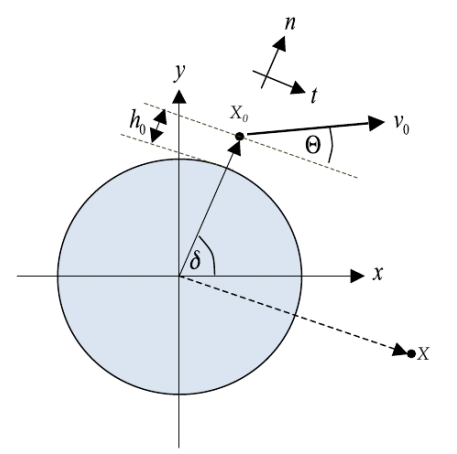
\includegraphics[width=0.5\linewidth]{./1_BezeichnerDiagramm}
\caption{}
\label{fig:1_BezeichnerDiagramm}
\end{figure}

\subsection{Gegebene Formeln und Konstanten}
Kraft auf den Satelliten
\begin{align}
\vec{F}_{S} = G \cdot \dfrac{m_{E} \cdot m_{S}}{r^2} \cdot \vec{e}_{SE}
\end{align}

Erdradius
\begin{align}
r_{E} = 6378 km
\end{align}

Erdmasse
\begin{align}
m_{E} = 5,9736 \cdot 10^{24} kg
\end{align}

Gravitationskonstante
\begin{align}
G = 66,743 \cdot 10^{-12} m^{3} kg^{-1} s^{-2}
\end{align}

\subsection{Konfigurierbare Parameter}
Folgende Parameter müssen mindestens bei der Simulation konfigurierbar sein:
\begin{itemize}
\item $v_{0}$ Startgeschwindigkeit $[km/s]$
\item $\Theta$ Flugwinkel $[^\circ]$
\item $\delta$ Startwinkel $[^\circ]$
\item $h_{0}$ Starthöhe $[km]$
\end{itemize}

\subsection{Erdachte Formeln}
Folgende Formeln wurden selbst erdacht, und sollen bei der Lösung behilflich sein:
\begin{align}
r = \sqrt{x^2 + y^2} \\
h = r - r_{E} \\
\vec{e}_{SE} = \dfrac{1}{\sqrt{x^2 + y^2}}\cdot \begin{pmatrix}x\\y\end{pmatrix} = \dfrac{1}{r} \cdot \begin{pmatrix}x\\y\end{pmatrix}
\end{align}

\subsection{Hinweise bei der Lösung mit MatLab}
\begin{itemize}
\item Die Simulation soll den Namen \textit{Erdorbits} haben.
\item In den Simulink-Schaltbildern sollen Vektorintegratoren verwendet werden. Das ist ein einfacher Integrator, der sein Eingangssignal aus einem Multiplexer erhält.
\item Die errechneten Bahnkoordinaten des Satelliten sollen von Simulink als getrennte x- und y-Werte in den MatLab-Workspace übergeben werden. Von dort werden sie visualisiert.
\item Sobald der Satellit die Erdoberfläche erreicht ($h=0$), soll die Simulink-Simulation beenden.
\item Es soll eine EM-Funktion \textit{Startposition} geben, die aus den Parametern $\gamma$, $h_{0}$ und dem Erdradius den Startpositionsvektor $x_{0}$ berechnet.
\item Es soll eine EM-Funktion \textit{vStart} geben, die aus $v_{0}$, $\Theta$ und $x_{0}$ soll der Startgeschwindigkeitsvektor berechnet werden. Der Vektor soll den Anfangswert als Weltkoordinaten enthalten. Dabei wird der Tipp gegeben, erst die Einheitsvektoren in Tangential- und Normalenrichtung ($\vec{n},\vec{t}$) aus $x_{0}$ zu konstruieren. Danach werden die Tangential- und Normalenkomponenten der Startgeschwindigkeit ($v_{t}$,$v_{n}$) berechnet. Abschließend wird aus den Einheitsvektoren und den Geschwindigkeitsvektoren die Bewegung des Satelliten berechnet.
\item Es soll eine EM-Funktion \textit{Beschleunigung} geben, die aus der aktuellen Satellitenposition $\vec{x}$ die aktuelle Satellitenbeschleunigung berechnet.
\item Es soll eine EM-Funktion \textit{Kontakt} geben, die den Wert \textit{0} ausgibt, solange der Satellit sich über der Erdoberfläche befindet ($h > 0$), ansonsten gibt sie den Wert \textit{1} aus.
\item Die Simulink-Simulation soll ein Display haben, dass die bislang vergangene Zeit in Stunden anzeigt.
\end{itemize}

\subsection{Durchführung 1}
Im ersten Experiment sollen die Werte $\gamma = 30^\circ,\ h_{0} = 400km$ und $\Theta=0^\circ$ angenommen werden. Die Startgeschwindigkeit $v_{0}$ soll so bestimmt werden, dass der Satellit in einer Kreisbahn auf gleicher Höhe fliegt (Tipp: ca. $7,4 - 8,5 km \dot s^{-1}$). Außerdem soll bestimmt werden, wie lange eine Erdumkreisung dann dauert (Tipp: ca. $1 - 2h$).

\subsection{Durchführung 2}
Im zweiten Experiment sollen die Werte $\gamma = 30^\circ,\ h_{0} = 400km$ und $\Theta=0^\circ$ angenommen werden und die Simulationszeit beträgt $1 \cdot 10^6s$. Es soll $v_{0}$ bestimmt werden, sodass der Satellit gerade der Erde entflieht (Tipp: ca. $10 - 11 km \cdot s^{-1}$).

\subsection{Durchführung 3}
Im dritten Experiment sollen die Werte $\gamma = 30^\circ$ und $\Theta = 0^\circ$ angenommen werden. Es sollen $h_{0}$ und $v_{0}$ so bestimmt werden, dass die Kreisbahn des Satelliten genau 1 Tag dauert. (Tipp: $h_{0} \approx 40000 km$ und $v_{0} \approx 3 km \cdot s^{-1}$)

\subsection{Hinweis zu Durchführungen}
Die Ergebnisse der Experimente können entweder durch Ausprobieren im Modell erreicht werden, oder durch Berechnung mit einer Formel.

%TODO: Es fehlt ein Diagramm das zeigt, wie der Mond zur Erde besteht und wie der Winkel dort benannte wird.
\section{Teilaufgabe 2}
Zu dieser Teilaufgabe wird das Simulink-Modell aus Teilaufgabe 1 kopiert. Nun soll der Satellit nicht mehr um die Erde kreisen, sondern zusätzlich auch um den Mond.

Zur Visualisierung des Modells wurde ein MatLab-Skript \textit{ErdMondBahn.m} bereitgestellt.

\subsection{Zusätzliche Konstanten}
Mondposition(fest)
\begin{align}
x_{M} = (0,-380000)^T km
\end{align}

Mondmasse
\begin{align}
m_{M} = 7,3480 \cdot 10^{22} kg
\end{align}

\subsection{Änderungen am Modell}
Im kopierten Simulink-Modell muss die EM-Funktion \textit{Beschleunigung} angepasst werden. %TODO: Wie muss sie angepasst werden?
Die Simulationszeit wird nun nicht mehr in Stunden, sondern in Tagen angegeben.

\subsection{Durchführung}
Es sind die Werte $\gamma_{0} = 30^\circ$ und $h_{0} = 150km$ gegeben.

Es müssen die Werte $v_{0}$ und $\Theta$ bestimmt werden, sodass der Satellit in einer 8-förmigen Schleife von der Erde startend um den Mond fliegt und zur Erde zurück fliegt. Es ist zu ermitteln, wie lange die Mission dauert.

\section{Teilaufgabe 3}
In dieser Teilaufgabe gilt es, die Bewegung einer Pendelkonstruktion zu berechnen. Der Versuchsaufbau ist in Abb. \ref{fig:3_Versuchsaufbau} zu sehen. In diesem Aufbau übt immer nur eine der Federn Zugkraft auf die Seiltrommel aus, während die andere Feder keine Kraft ausübt. Befindet sich das Pendel in senkrechter Position, dann übt keine der Federn eine Kraft aus. Der Einfluss der Pendelstange und der Seiltrommel werden nicht beachtet.

\begin{figure}[H]
\centering
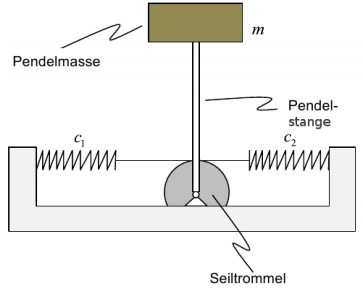
\includegraphics[width=0.5\linewidth]{./3_Versuchsaufbau}
\caption{}
\label{fig:3_Versuchsaufbau}
\end{figure}

\subsection{Konfigurierbare Parameter}
Es sind folgende Parameter in der Simulation konfigurierbar:
\begin{itemize}
\item Pendelmasse $m$[kg]
\item Abstand $L$[m]
\item Quadermaße $w$[m] und $h$[m]
\item Trommelradius $r$ [m]
\item Auslenkung des Pendels zu Versuchsbeginn $\varphi$[$^\circ$]
\item Federkonstanten $c_{1}$[N/m] und $c_{2}$[N/m]
\end{itemize}

\subsection{Ausgabe der Simulation}
Das Ergebnis der Simulation soll $varphi(t)$ sein. Die erhaltenen Werte sollen als Graph im Koordinatensystem, sowie als virtuelles Modell visualisiert werden.

Für das virtuelle Modell wird eine WRL-Datei bereitgestellt, die man in Simulink integrieren kann.

\subsection{Hinweise bei der Modellierung}
Bevor die Simulation in MatLab nachgestellt wird, sind zuvor einige Dinge zu tun.

In einem Freikörperbild des Pendels sollen die angreifenden Kräfte angetragen werden. Dazu gehört die Erdanziehungskraft, die man mithilfe von $varphi$ in ihre Tangetial- und Normalenkomponenten zerlegen kann, und das jeweils angreifende Drehmoment.

Außerdem muss das Massenträgheitsmoment für die quaderförmige Pendelmasse angegeben werden.

Dann muss eine DGL aufgestellt werden, die die Bewegung des Pendels berechnet.

Zum Schluss muss das Modell in Simulink abgebildet werden.

\subsection{Versuchsdurchführung}
Der Versuch wird unter folgenden Randbedingungen durchgeführt: $L=1m,\ m=10kg,\ r=0.3m,\ w=0.3m,\ h=0.2m,\ c_{1}=5000N/m,\ c_{2}=500\ 000N/m,\ \varphi(0)=45^\circ$
Es ist das resultierende $\varphi(t)$ als Graph darzustellen.

Außerdem ist die bereits erwähnte \textit{CrazyPendlm.wrl} in Simulink zu integrieren, um das virtuelle Modell zu erhalten. Es ist darauf zu achten, dass die Sample-Time der VR-Sind auf 0.005 gesetzt wird.

\section{Teilaufgabe 4}
In dieser Teilaufgabe wird ein schwingungsgedämpfter Tisch simuliert. Der Versuchsaufbau ist in Abb. \ref{fig:4_Versuchsaufbau} zu sehen. Der Startbewegungsimpuls wird über \textit{u} gegeben. Die Massen $m_{1}$ und $m_{2}$ reagieren darauf mit den Auslenkungen $x_{1}$ und $x_{2}$.

\begin{figure}[H]
\centering
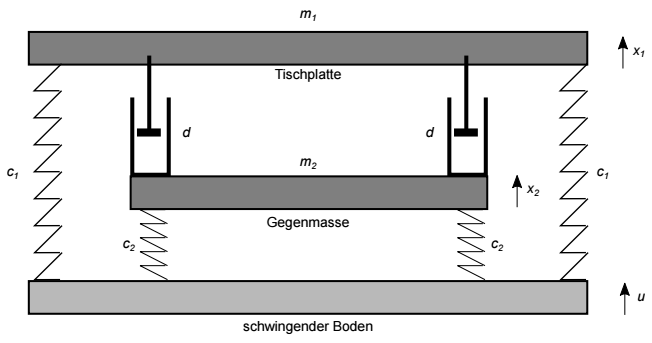
\includegraphics[width=0.5\linewidth]{./4_Versuchsaufbau}
\caption{}
\label{fig:4_Versuchsaufbau}
\end{figure}

\subsection{Konfigurierbare Parameter}
Es sind folgende Parameter in der Simulation konfigurierbar:
\begin{itemize}
\item Tischplattenmasse $m_{1}$[kg]
\item Gegenmasse $m_{2}$[kg]
\item Federkonstante $c_{1}$[N/m]
\item Federkonstante $c_{2}$[N/m]
\item Dämpfer $d$[Ns/m]
\end{itemize}

\subsection{Ausgabe der Simulation}
Das Ergebnis der Simulation soll der Graph von $x_{1}(t)$ sein.

\subsection{Hinweise bei der Modellierung}
Zunächst müssen an einem Freikörperbild alle angreifenden Kräfte angetragen werden. In diesem Versuch gibt es ausschließlich senkrecht wirkende Kräfte. Dazu gehören jeweils die Erdanziehungskräfte, die auf die Massen $m_{1}$ und $m_{2}$ wirken. Außerdem die Kräfte der Federn, die jeweils in Richtung Boden ziehen. Zuletzt gibt es die Kräfte der Dämpfer, die beiden Massen "auseinander drücken".

Außerdem sind die DGLn für die Massen $m_{1}$ und $m_{2}$ aufzustellen und die Ruhelagen der Massen zu bestimmen. Das ist der Moment, wenn in dem Versuchsaufbau keine Bewegung mehr stattfindet und alle Kräfte ausgeglichen sind.

\subsection{Versuchsdurchführung}
Der Versuch wird unter folgenden Randbedingungen durchgeführt: $c_{1} = 15\ 000N/m,\ c_{2}=10\ 000N/m,\ d=600Ns/m,\ m_{1}=60kg,\ m_{2}=450kg$
Es ist das resultierende $x_{1}(t)$ als Graph darzustellen.

Die Startbewegung des Versuchs ist $u=1mm$.

\end{document}
